\chapter{Compressed suffix arrays}\label{chapter:csa}

\section{Original indexes}\label{sect:original indexes}

The \emph{compressed suffix arrays (CSA)} discussed in this chapter are compressed self-indexes that provide the functionality of the suffix array (Definition~\ref{def:suffix array}). They are based on backward searching on the Burrows-Wheeler transform (see Section~\ref{sect:full-text indexes}), with their major differences in the solutions used to encode the BWT and support $rank$ and $select$ on it.

The first index in the CSA family was the compressed suffix array of Grossi and Vitter \cite{Grossi2005}. It was not a self-index, but encoded the suffix array of text $T[1,n]$ recursively in the following way:
\begin{itemize}

\item Binary string $B[1,n]$ is used to mark even suffix array values: $B[i] = 1$, if $\SA[i]$ is even.

\item For odd suffix array values $\SA[i]$, we store $\Psi(i)$ instead. As $\Psi$ is strictly increasing in range $C_{c}$ for all $c \in \Sigma$, these values form $\sigma$ increasing sequences that can be encoded efficiently by using gap encoding (see Section~\ref{sect:bit vectors}). If odd $\SA[i]$ is needed, it can be computed as $\SA[\Psi(i)] - 1$.

\item For even suffix array values $\SA[i]$, we store $\SA[i] / 2$ in array $\SA'$. If even $\SA[i]$ is needed, it can be computed as $2 \cdot \SA'[rank_{1}(B, i)]$. Array $\SA'$ can either be stored explicitly or encoded recursively.

\end{itemize}
Sadakane later transformed the compressed suffix array into a self-index \cite{Sadakane2003}, and showed how to implement backward searching using $\Psi$ instead of $\BWT$ \cite{Sadakane2002}.

The \emph{FM-index (FMI)} of Ferragina and Manzini \cite{Ferragina2005a} was a simultaneous development that was already a self-index. The BWT was split into blocks that were compressed separately. To support backward searching, the $\mrank_{c}(\BWT, \cdot)$ value corresponding to the beginning of each block was stored explicitly for each character $c$. To compute $rank$ for later positions, the block had to be decompressed. Later developments concentrated on improving the time/space trade-offs for large alphabets.

Because of these historical roots, papers on indexes of the CSA family still often discuss compressing $\Psi$, while papers on the FMI family discuss compressing the BWT. This is not a fundamental distinction, however. As function $\Psi$ is strictly increasing in range $C_{c}$ for all characters $c \in \Sigma$, we can represent this part of $\Psi$ as a binary string $B_{c}$, where $B_{c}[i] = 1$ if and only if $\Psi(j) = i$ for some $j \in C_{c}$. But as $\Psi(j) = \mselect_{c}(\BWT, j - C[c])$, where $j \in C_{c}$, this means that $B_{c}[i] = 1$ if and only if $\BWT[i] = c$. As most indexes in the CSA family store the values of $\Psi$ separately for each of the ranges $C_{c}$, they are essentially encoding the BWT by binary strings $B_{c}$. Hence the differences between the CSA family and the FMI family are more semantical than technical in nature.

We describe the CSA family, based on encoding the binary strings $B_{c}$, in more detail in Section~\ref{sect:bit vectors}. Section~\ref{sect:wavelet trees} discusses the FMI family, concentrating on supporting $rank$ and $select$ directly on $\BWT$ by using wavelet trees. There are also other proposals \cite{Golynski2006,Barbay2010,Li2009} to support $rank$ and $select$ on $\BWT$ that we will not consider here. Later sections describe the techniques used to support \locate\ and \extract, as well as dynamic compressed suffix arrays that allow various updates to the text.

In addition to the compressed suffix arrays, there are also compressed indexes that are based on Lempel-Ziv parsing of the text \cite{Navarro2004,Ferragina2005a,Russo2008a,Kreft2011}. In general, these \emph{\lzindex{}es} have faster \locate\ and \extract\ than the BWT-based indexes \cite{Ferragina2009a}. On the other hand, they do not support \find, as they are not based on compressing the suffix array. These \lzindex{}es are not further discussed in the thesis.


\section{CSA family}\label{sect:bit vectors}

\paragraph{Bit vectors.}

\emph{Bit vectors} are the basic building block of compressed data structures. Built for a binary sequence $B[1,n]$, a bit vector provides efficient support for operations $rank_{1}(B, \cdot)$ and $select_{1}(B, \cdot)$. Some structures also support $select_{0}(B, \cdot)$, while $rank_{0}(B, \cdot)$ can be solved by reduction $rank_{0}(B, i) = i - rank_{1}(B, i)$. In the following, bit vector $B$ refers both to the binary sequence and the data structure.

Indexes of the CSA family use bit vectors $B_{c}$, where $B_{c}[i] = 1$ if and only if $\BWT[i] = c$, to represent the BWT. They reduce the basic operations $rank_{c}(\BWT, \cdot)$ and $select_{c}(\BWT, \cdot)$ to $rank_{1}(B_{c}, \cdot)$ and $select_{1}(B_{c}, \cdot)$, respectively. The best encoding for the bit vectors depends on the type of data, the size of the alphabet, and the desired time/space trade-off.

A basic succinct bit vector \cite{Jacobson1989,Munro1996,Clark1996} consists of the binary sequence and separate $o(n)$\nobreakdash-bit indexes for $rank$ and $select$. For $rank$, we split the sequence into \emph{large blocks} of $l = \log^{2} n$ bits, and store the number of \onebit{}s before each block in array $R_{l}$. A large block is further divided into \emph{small blocks} of $s = \log n / 2$ bits, and the number of \onebit{}s in previous small blocks of the same large block is stored in array $R_{s}$. These arrays take $O(n / \log n)$ and $O(n \log \log n / \log n)$ bits, respectively. We can now solve
$$
rank_{1}(B, i) = R_{l}[\lfloor i / l \rfloor] + R_{s}[\lfloor i / s \rfloor] + \popcount(B[s \cdot \lfloor i / s \rfloor, i]),
$$
where $\popcount(S)$ is the number of \onebit{s} in sequence $S$, in constant time. In practice, this solution requires $3$ or $4$ random memory accesses per $rank$, depending on whether $\popcount$ is solved directly or by using lookup tables.

In \select, large and small blocks consist of $\kappa = \log^{2} n$ \onebit{}s and $\log^{2} \kappa = O((\log \log n)^{2})$ \onebit{}s, respectively. Arrays similar to $R_{l}$ and $R_{s}$ in \rank\ are used to store the answer to \select\ for the first \onebit{} of each block. These arrays take $O(n / \log n)$ bits for large blocks and $O(n / \log \log n)$ bits for small blocks. A lookup table is used to answer \select\ for the \onebit{}s within a small block. This solution takes $O(1)$ time and up to $4$ random memory accesses.

An exception to the above are long blocks. If a large block spans more than $\log^{4} n$ positions in the sequence, relative positions within it might take more than $O(\log \log n)$ bits each. But as there are at most $O(n / \log^{2} n)$ \onebit{}s within such blocks, we can store their positions explicitly in $O(n / \log n)$ bits and ignore the small blocks. Similarly, if a small block spans more than $\log n$ positions, answering \select\ within it might not be constant-time. Yet as there are at most $O(n (\log \log n)^{2} / \log n)$ \onebit{}s within these blocks, storing their relative positions takes at most $O(n (\log \log n)^{3} / \log n)$ bits.

As there are $\binom{n}{n_{1}}$ binary sequences of length $n$ with $n_{1}$ \onebit{}s, we can store the sequence in $\lceil \log \binom{n}{n_{1}} \rceil \le \lceil nH_{0} \rceil$ bits. A simple entropy-compressed bit vector achieves $nH_{0} + o(n)$ bits of space by storing each small block as a pair of integers $(i, j)$, where $i$ is the number of \onebit{}s in the block, and $j$ is the lexicographic rank of the block among those blocks with $i$ \onebit{}s. The bit vector of Raman \etal{Raman2002} requires $nH_{0} + O(n \log \log n / \log n)$ bits of space, and supports $rank$ and $select$ in constant time.

An alternative approach is to use \emph{gap encoding} (also called \emph{differential encoding}) to compress the sequence. Each \onebit{} is stored as the distance between it and the previous \onebit, often by using \gammacode{}s or \deltacode{}s. Indexes are built for large and small blocks to allow fast decoding. The relevant complexity metric here is 
$$
\gap(B) = \sum_{i=1}^{n_{1}} \lceil \log(select_{1}(B, i) - select_{1}(B, i-1) + 1) \rceil,
$$
where $select_{1}(B, 0) = 0$. If the sequence is evident from the context, we write $\gap$ instead of $\gap(B)$, as with the other complexity metrics. In the worst case, we have $\gap \lessapprox n_{1} \log (n / n_{1}) \le nH_{0}$, but $\gap$ can get much smaller, if the \onebit{}s are not evenly spaced \cite{Gupta2007}.\footnote{A pessimistic non-approximate bound is $\gap \le n_{1} \log (n / n_{1}) + n_{1}$.} The bit vector of Gupta \etal{Gupta2007} achieves sublogarithmic query complexity, while its space occupancy is $\gap + O(n_{1} \log (n / n_{1}) / \log n_{1}) + O(n_{1} \log \log (n / n_{1}))$ bits.

Gap encoding essentially replaces \emph{runs} of \zerobit{}s with their lengths. If there are long runs of \onebit{}s, it may be beneficial to replace these runs as well. This technique is called \emph{run-length encoding (RLE)}. Bit vectors can use RLE directly or reduce it to gap encoding. One such reduction replaces binary sequence $B$ with another sequence $B'$ that contains an \onebit{} at the first position of every run of \zerobit{}s and \onebit{}s in $B$. The relevant complexity metrics are the number of runs of \onebit{}s $R(B)$ (or just $R$) and $\run(B) = \gap(B')$. In the worst case, $\run(B) \lessapprox 2R(B) \log (n / (2R(B)))$ by the same reasoning as with gap encoding.

\paragraph{Choosing the bit vector.}

The choice between various encodings depends on the sequence $B$ (see Okanohara \etal{Okanohara2007}). If $B$ is essentially random, succinct representation and entropy compression are both good choices. For $n_{1} \approx n/2$, we have $H_{0} \approx 1$, and both representations achieve similar size. On the other hand, if the distribution is biased, entropy compression can reduce the size significantly. For non-random $B$, gap encoding or run-length encoding may be able to exploit the structure at the cost of query performance. Note that while entropy compression and gap encoding both have $nH_{0}$ as the most significant term in their size bounds, their actual performances differ. For a \emph{sparse} sequences, where $n_{1} \ll n/2$, gap encoding is often a better choice, as it usually has larger small blocks and hence less overhead. Entropy compression tends to perform better in \emph{dense} (non-sparse) sequences, as gap encoding has some overhead per \onebit{}.

When the sequence $B$ is very compressible, low-order terms in the size bound can dominate the size of the bit vector. For example, the $O(n \log \log n / \log n)$ term of the bit vector of Raman \etal{Raman2002} is almost linear in $n$, so it dominates the overall size when $H_{0} \ll 1$. In these cases, it is preferable to use a \emph{data-aware} bit vector, where the size overhead scales  either with the compressed size of the sequence or with some related property of the sequence. An example of a data-aware bit vector is the one by Gupta \etal{Gupta2007}, with the low-order term almost linear in the number of \onebit{}s $n_{1}$. The key for making a bit vector data-aware is to make the small blocks data-aware: they might contain a certain amount of compressed data or a certain number of \onebit{}s.

The size of gap encoded and run-length encoded bit vectors depends greatly on the integer codes they use. A common solution is to use either \gammacode{}s or \deltacode{}s. While \deltacode{}s are asymptotically smaller, \gammacode{}s have smaller code lengths for integers $i \in \set{2, 3, 8, \dotsc, 15}$. For $i \ge 32$, \deltacode{}s are shorter than \gammacode{}s. When used in compressed suffix arrays, \gammacode{}s perform better for regular texts \cite{Foschini2006}, while \deltacode{}s are better for low-entropy or highly repetitive texts \cite{Grossi2011}.

\paragraph{Self-indexes of the CSA family.}

Assume that we want to use a bit vector that supports \rank\ in time $t_{R}$ and \select\ in time $t_{S}$ to encode the binary sequences $B_{c}$. To compute $\Psi(i)$, we must be able to determine efficiently the largest character $c$ with $C[c] < i$. One solution is to use bit vector $C'$, where $C'[i] = 1$ if $C[c] = i$ for some character $c > 0$.\footnote{This solution assumes that every character of alphabet $\Sigma$ appears in the text.} Then $\Psi(i) = \mselect_{1}(B_{c'}, i - C[c'])$, where $c' = \mrank_{1}(C',i)$. Hence $\Psi$ can be computed in $t_{\Psi} = O(t_{R} + t_{S})$ time.

For backward searching, we need to compute $LF$ for the first and the last occurrences of character $P[i-1]$ in range $\BWT[sp_{i},ep_{i}]$. This can be done as
\begin{align*}
sp_{i-1} & = C[P[i-1]] + \mrank_{1}(B_{P[i-1]}, sp_{i}-1) + 1; \\
ep_{i-1} & = C[P[i-1]] + \mrank_{1}(B_{P[i-1]}, ep_{i}).
\end{align*}
Hence one step of backward searching takes $t_{B} = O(t_{R})$ time.

\begin{theorem}[From Theorems \ref{theorem:backward searching} and \ref{theorem:full functionality}]\label{theorem:csa}
Let \rank\ and \select\ on binary sequences take $t_{R}$ and $t_{S}$ time, respectively. Then a self-index of the CSA family with sample rate $d$ supports \find$(P)$ in $O(\abs{P} \cdot t_{R})$ time, \locate\ in $O(d \cdot (t_{R} + t_{S}))$ time, and \extract$(i,j)$ in $O((d + j - i)(t_{R} + t_{S}))$ time.
\end{theorem}

See Section~\ref{sect:full functionality} for the definition of sample rate $d$.

To compute $LF(i)$ for an arbitrary position $i$, we need to know the character $\BWT[i]$. As the character can be encoded in any of the binary sequences $B_{c}$, this takes $t_{LF} = O(\sigma \cdot (t_{R} + t_{S}))$ time. Hence computing $LF$ is inefficient in the CSA family, except for sequences with small alphabets.

As the encoding of $\BWT$ consists of $\sigma$ bit vectors of length $n$, any $o(n)$\nobreakdash-bit terms in the size bound of the bit vector will sum up to $o(\sigma n)$ bits. In practice, this can be much more than the $n \log \sigma$ bits of the original sequence. Hence indexes of the CSA family tend to use bit vectors that are at least partially data-aware, with non-constant \rank\ and/or \select\ times.

The best-known index of the CSA family is the \emph{compressed suffix array of Sadakane (\sadcsa)} \cite{Sadakane2003,Sadakane2002}. It uses a differential encoding of $\Psi$ that is essentially either a gap encoded or a run-length encoded representation of the bit vectors $B_{c}$. A run-length encoded \sadcsa{} requires $nH_{k} + O(n \log \log \sigma)$ bits for $k \le \alpha \log_{\sigma} n$ and some constant $0 < \alpha < 1$ \cite{Navarro2007}. The performance of \sadcsa\ follows from Theorems \ref{theorem:backward searching} and \ref{theorem:full functionality} with $t_{B} = O(\log n)$, $t_{R} = t_{S} = O(1)$, and $t_{\Psi} = O(1)$. In practice, Sad-CSA provides good compression and supports \locate\ and \extract\ very efficiently, while losing to other indexes in \find\ \cite{Ferragina2009a}.

The \emph{run-length compressed suffix array (RLCSA)} \cite{Maekinen2010,Siren2009} uses data-aware run-length encoded bit vectors to encode the sequences $B_{c}$. Intended for indexing highly repetitive sequences, RLCSA requires
$$
R
\left( \log \frac{\sigma n}{R} + \log \frac{n}{R} + O\left( \log\log \frac{\sigma n}{R} \right) \right)
\left( 1 + \frac{O(\log n)}{b} \right) +
O(\sigma \log n)
$$
bits of space, where $b$ is the block size in bits. For $b = O(\log n)$, the performance follows from Theorem~\ref{theorem:csa} with $t_{R} = t_{S} = O(\log n)$. This index is described in detail in Chapter~\ref{chapter:rlcsa}.


\section{FMI family}\label{sect:wavelet trees}

\paragraph{Wavelet trees.}

The \emph{wavelet tree} \cite{Grossi2003} is a versatile data structure that supports \rank\ and \select\ on general sequences. In its general form \cite{Ferragina2007a}, a wavelet tree reduces \rank\ and \select\ on strings over alphabet $\Sigma$ to the same operations on strings over a smaller alphabet $\Sigma'$. An example of a wavelet tree can be seen in Figure~\ref{fig:wavelet tree}.

\begin{figure}
\centerline{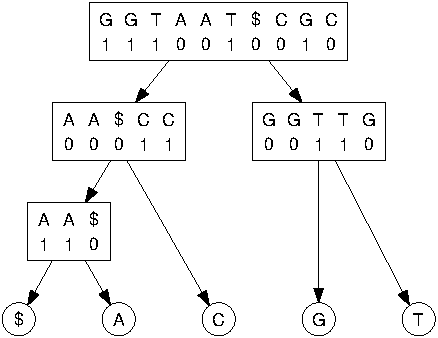
\includegraphics{figures/wavelet.pdf}}
\caption{A binary wavelet tree for sequence \texttt{GGTAAT\${}CGC} (the Burrows-Wheeler transform in Figure~\ref{fig:suffix structures}). The internal nodes of an actual wavelet tree contain only the binary sequences, but not the conceptual character sequences.}
\label{fig:wavelet tree}
\end{figure}

\begin{definition}
A wavelet tree for string $S$ over alphabet $\Sigma$ with internal alphabet $\Sigma'$ is a rooted tree, where each internal node has at most $\abs{\Sigma'}$ children, and the leaves are the characters of alphabet $\Sigma$. Let $v_{1}, \dotsc, v_{k}$ be the children of the root node. The root is labeled with string $S'$, where $S'[i] = j$, if character $S[i]$ is in the subtree with $v_{j}$ as its root. The subtree of each child $v_{j}$ is a wavelet tree for the subsequence $S_{j}$ of $S$ that contains only the characters in that subtree.
\end{definition}

Let $v_{j}$ be the root of the subtree containing character $c$. With the above definition, \rank\ and \select\ over string $S$ are supported in the following way:
\begin{align*}
\mrank_{c}(S,i) & = \mrank_{c}(S_{j}, \mrank_{j}(S',i)); \\
\mselect_{c}(S,i) & = \mselect_{j}(S', \mselect_{c}(S_{j},i)).
\end{align*}
The computation of \rank\ starts at the root and proceeds towards the leaf, where $\mrank_{c}(S,i) = i$, while \select\ starts from the leaf with $\mselect_{c}(S,i) = i$ and proceeds towards the root. In either case, \rank\ or \select\ on string $S$ is reduced to $h$ operations with the internal alphabet, where $h$ is the distance of character $c$ from the root. Character $S[i]$ can also be determined in $h$ steps by starting from the root, continuing to the subtree of $v_{S'[i]}$, and searching for character $S_{S'[i]}[\mrank_{S'[i]}(S',i)]$ there.

\paragraph{Compression with wavelet trees.}

Burrows-Wheeler transform groups characters followed by the same $k$-character context together, simultaneously for all $k \ge 0$. If we partition $\BWT$ by \orderk{k} contexts for some fixed $k$, and encode each part separately by an \orderk{0} encoder, the result will be compressed to the \orderk{k} entropy of the reverse text, excluding low-order terms. Compression boosting \cite{Ferragina2005} improves upon this by finding the partition that minimizes the overall size for a given \orderk{0} encoder.

In practice, a quickly adapting \orderk{0} encoder uses an almost optimal partition implicitly, achieving similar compression as explicit boosting \cite{Ferragina2006a}. We can use this implicit compression boosting to achieve $nH_{k} + o(n \log \sigma) + O(\sigma^{k+1} \log n)$ bits of space simultaneously for all $k \ge 0$ by using the bit vector of Raman \etal{Raman2002} to encode a binary wavelet tree \cite{Maekinen2008a}. This means that, in some sense, indexes of the FMI family can achieve similar compression as the best BWT-based compressors.

\paragraph{Building the self-index.}

Assume that the wavelet tree is a complete binary tree, and the sequences are encoded by a bit vector supporting
\rank\ in time $t_{R}$ and \select\ in time $t_{S}$. Then we can compute $LF(i) = C[\BWT[i]] + \mrank_{\BWT[i]}(\BWT,i)$  with $\log \sigma$ \rank\ operations in $t_{LF} = O(t_{R} \log \sigma)$ time by recursion
$$
\mrank_{\BWT[i]}(\BWT,i) = \mrank_{\BWT[i]}(S_{S'[i]}, \mrank_{S'[i]}(S',i)).
$$
With array $C$ implemented in the same way as in the CSA family, we can compute $\Psi(i) = \mselect_{c}(\BWT, i - C[c])$ in $t_{\Psi} = O(t_{R} + t_{S} \log \sigma)$ time. A step of backward searching
\begin{align*}
sp_{i-1} & = C[P[i-1]] + \mrank_{P[i-1]}(\BWT, sp_{i}-1) + 1; \\
ep_{i-1} & = C[P[i-1]] + \mrank_{P[i-1]}(\BWT, ep_{i}).
\end{align*}
can be done in $t_{B} = O(t_{R} \log \sigma)$ time.

\begin{theorem}[From Theorems \ref{theorem:backward searching} and \ref{theorem:full functionality}]\label{theorem:fmi}
Let \rank\ and \select\ on binary sequences take $t_{R}$ and $t_{S}$ time, respectively. Then a self-index of the FMI family with sample rate $d$ supports \find$(P)$ in $O(\abs{P} \cdot t_{R} \log \sigma)$ time, \locate\ in $O(d \cdot t_{R} \log \sigma)$ time, and \extract$(i,j)$ in $O((d + j - i) \cdot t_{R} \log \sigma)$ time.
\end{theorem}

See Section~\ref{sect:full functionality} for the definition of sample rate $d$.

With a Huffman-shaped wavelet tree, we can replace the $\log \sigma$ factors in time complexities by the \orderk{0} entropy $H_{0}$ in the expected case \cite{Foschini2006}. Note that as the total length of the bit vectors is $n \log \sigma$, the sublinear terms in size bounds sum up to $o(n \log \sigma)$. Hence, unlike in the CSA of Theorem~\ref{theorem:csa}, we can use the bit vectors with $t_{R} = t_{S} = O(1)$ to overcome the extra $\log \sigma$ factors in time complexities.

\paragraph{Self-indexes of the FMI family.}

The \emph{succinct suffix array (SSA)} \cite{Maekinen2005} is a simple Huffman-shaped wavelet tree using succinct bit vectors with $t_{R} = t_{S} = O(1)$. It requires $n(H_{0}+1)(1+o(1))$ bits of space, and its performance follows from Theorem~\ref{theorem:fmi}. In practice, SSA is one of the fastest self-indexes, due to its simplicity \cite{Ferragina2009a}. However, other indexes achieve better compression on texts with low high-order entropy.

The \emph{run-length FM-index (RLFM)} \cite{Maekinen2005} is a variant of the SSA that builds the wavelet tree over the \emph{run heads} (the first characters of each run) of the BWT, and uses a separate bit vector to encode the lengths of the runs. Its performance follows from Theorem~\ref{theorem:fmi} with $t_{R} = t_{S} = O(1)$, while the size bound is $nH_{k} \log \sigma + 2n + o(n \log \sigma)$ bits for $k \le \log_{\sigma} n - \omega(1)$. In practice, the query performance of RLFM is similar to AFFM below \cite{Claude2008}. Index size tends to be larger than AFFM on regular texts \cite{Claude2008} and smaller on highly repetitive texts \cite{Siren2008}. A data-aware variant of RLFM exists, but it is both larger and slower than RLCSA \cite{Maekinen2010}.

Instead of a single wavelet tree, the \emph{alphabet-friendly FM-index (AFFM)} \cite{Ferragina2007a} uses explicit compression boosting to partition the BWT, and encodes each part separately with a wavelet tree with internal alphabet of size $o(\log n / \log \log n)$. Compression boosting guarantees a size bound of $nH_{k} + o(n \log \sigma)$ bits for $k \le \alpha \log_{\sigma} n - 1$, while the performance of AFFM follows from Theorems \ref{theorem:backward searching} and \ref{theorem:full functionality} with $t_{B} = t_{LF} = O(1 + \log \sigma / \log \log n)$ and $t_{R} = t_{S} = O(1)$. AFFM achieves similar compression as \sadcsa, with fast \find\ and relatively slow \locate\ and \extract\ \cite{Ferragina2009a}.

There are several variants of SSA using compression boosting. With the implicit compression boosting offered by the bit vector of Raman \etal{Raman2002} on a balanced wavelet tree, we get the same size bound as for AFFM. The query performance of this FMI variant follows from Theorem~\ref{theorem:fmi} with $t_{R} = t_{S} = O(\log \sigma)$. Another variant (\ssarrr) using a Huffman-shaped tree improves both size and performance, making the index smaller than AFFM and RLFM, but also slower than them \cite{Claude2008}. We get the same size bound by dividing the BWT into blocks of $\sigma \log^{2} n$ characters and building a separate SSA or \ssarrr\ for each of the blocks \cite{Kaerkkaeinen2011}. With \ssarrr\ as the basic index, this variant is the smallest entropy-compressed index of the FMI family, and almost as fast as AFFM. When using SSA, we combine the size of AFFM with the performance of SSA. 

A data-aware run-length encoded variant of SSA also exists \cite{Maekinen2010}. While this index offers slightly better compression than RLCSA, it is much slower in practice.


\section{Supporting full functionality}\label{sect:full functionality}

\paragraph{Sampling mechanism.}

The basic solution to \locate\ and \extract\ has not changed much since the original FM-index \cite{Ferragina2005a}. We sample a number of pairs $(i, \SA[i])$, and use either $LF$ or $\Psi$ to derive the unsampled positions.

Assume that we want to retrieve $\SA[i]$. If suffix array position $i$ is sampled, we can just use the sampled value. Otherwise we compute $LF(i)$ and continue from that position. Eventually, after $k$ steps, we find a sample $(LF^{k}(i), \SA[LF^{k}(i)])$. As $\SA[LF(i)] = \SA[i] - 1$ (unless $\SA[i] = 1$), we now know that $\SA[i] = \SA[LF^{k}(i)] + k$. The special case can be avoided by always sampling $(\SA^{-1}[1], 1)$. In a similar way, we can also use $\Psi$ to find $\SA[i]$. As $\SA[\Psi(i)] = \SA[i] + 1$ (unless $\SA[i] = n$), we get $\SA[i] = \SA[\Psi^{k}(i)] - k$, where $(\Psi^{k}(i), \SA[\Psi^{k}(i)])$ is a sampled position.

To extract substring $T[i,j]$, we find the smallest $k \ge j$, for which $(SA^{-1}[k],k)$ has been sampled, and use $LF$ to proceed backwards. After $k - j$ steps, we have reached $(LF^{k-j}(\SA^{-1}[k]), j)$. We can now determine $T[j] = c$, where $C[c] < LF^{k-j}(\SA^{-1}[k]) \le C[c+1]$. After that, we proceed with $LF$ until we reach $T[i]$, and determine each character in the same way. Instead of using $LF$, we can also use $\Psi$ by starting at the largest sampled value $k \le i$ and moving forward until we reach $T[j]$.

A practical solution is to sample $(i, \SA[i])$ for those positions $i$, where $\SA[i] = j \cdot d$ for some \emph{sample rate} $d > 0$, in addition to the special cases $(\SA^{-1}[1],1)$ and $(1,n)$. Then the nearest sample is always within $d-1$ steps of $LF$ or $\Psi$. The sampled positions are marked in bit vector $B_{s}$ ($B_{s}[i] = 1$, if $(i, \SA[i])$ has been sampled). Sampled values are encoded as $\SA[i] / d$, taking $\log (n/d)$ bits each, and stored in array $\SA_{s}$ in suffix array order. Checking whether $\SA[i]$ has been sampled takes $O(t_{R})$ time, where $t_{R}$ is the time required to answer $\mrank_{1}(B_{s}, i)$. Retrieving a sampled value $\SA[i] = d \cdot \SA_{s}[\mrank_{1}(B_{s}, i)]$ also takes $O(t_{R})$ time.

For \extract, the starting position $k$ is $d \cdot (\lfloor (j-1) / d \rfloor + 1)$ when using $LF$ and $d \cdot \lfloor i / d \rfloor$ when using $\Psi$. For all samples $(\SA^{-1}[k], k)$, we store the values $\mrank_{1}(B_{s}, \SA^{-1}[k])$ in an array in text order. This array $\SA^{-1}_{s}$ takes a total of $(n/d) \log (n/d)$ bits. We can determine $\SA^{-1}[k] = \select_{1}(B_{s}, \SA^{-1}_{s}[k / d])$ for a sampled text position $k$ in $O(t_{S})$ time, where $t_{S}$ is the time required to answer \select. The current character can be determined in $O(t_{R})$ time by using the bit vector representation of array $C$.

\begin{theorem}\label{theorem:full functionality}
Assume that an index computes $LF$ in $t_{LF}$ time and $\Psi$ in $t_{\Psi}$ time, and that we are given a bit vector that supports \rank\ in $t_{R}$ time and \select\ in $t_{S}$ time. Then we can answer \locate\ in $O(d \cdot (t_{R} + \min(t_{LF}, t_{\Psi})))$ time and extract substring $T[i,j]$ in $O(t_{S} + (d + j - i)(t_{R} + \min(t_{LF}, t_{\Psi}))$ time by using $O((n/d) \log (n/d)) + \abs{B}$ bits of extra space, where $d > 0$ is the sample rate and $\abs{B}$ is the size of the bit vector.
\end{theorem}

In theoretical size bounds, the sample rate is often assumed to be $\log^{1+\varepsilon} n$ for some $\varepsilon > 0$. Then, assuming that we use the bit vector of Raman \etal{Raman2002} for marking the sampled positions, the extra space becomes $o(n)$ bits, while $t_{R} = t_{S} = O(1)$.

\paragraph{Optimizations.}

If the index supports both $LF$ and $\Psi$ efficiently (as the FMI family does), we can effectively double the number of samples by using an extra binary string $B_{n}$ of length $n$. For each suffix array position $i$, we write $B_{n}[i] = 1$, if the nearest sample can be found faster by using $\Psi$ than by using $LF$. This reduces the expected distance to the nearest sample from $d/2$ to $d/4$. If $d \approx \log n$, this is already more space-efficient than doubling the number of samples.

A typical use of \locate\ is to call it for all positions in the suffix array range returned by \find. If the text is repetitive, it can be more efficient to compute \locate\ for all positions in the range simultaneously, instead of doing it one position at a time. If suffix array positions $i$ and $i+1$ are located in the same equal letter run in BWT (self-repetition in the suffix array), then $LF(i+1) = LF(i) + 1$ ($\Psi(i+1) = \Psi(i) + 1$), and the corresponding bit vector operations are usually faster than for arbitrary positions. In repetitive texts, positions $LF(i)$ and $LF(i+1)$ ($\Psi(i)$ and $\Psi(i+1)$) are also in the same run (self-repetition) with high probability, and a significant amount of work can be saved by doing \locate\ simultaneously for the entire range. See Section~\ref{sect:rlcsa experiments} for experimental results.

The standard sampling strategy, as described above, is geared towards worst case performance. As the nearest sample is never more than $d-1$ steps away, the desired position can be found in $O(d \cdot t_{LF})$ or $O(d \cdot t_{\Psi})$ time. On the other hand, if the query distribution is very skewed, another sampling strategy might provide better expected case performance. Experiments suggest that \locate\ can be up to $10$ times faster, if the samples have been optimally selected for a known distribution \cite{Ferragina2011}.\footnote{The full version of \cite{Ferragina2011} reports even greater speedups.} Adapting the samples for an unknown query distribution remains an open problem.


\section{Dynamic versions}\label{sect:dynamic indexes}

Consider the differences between the Burrows-Wheeler transforms of texts $T$ and $cT$, for an arbitrary text $T$ and an arbitrary character $c$. In both cases, the position of the end marker, $\mrank(T,T)$ or $\mrank(cT,cT)$, is determined by the longest suffix. Additionally, $\BWT_{cT}[\mrank(cT,T)] = c$, while $\BWT_{T}[\mrank(T,T)] = \$$. This suggests of a simple procedure for obtaining $\BWT_{cT}$ from $\BWT_{T}$ (see Figure~\ref{fig:bwt update}). The first step is essentially a step of backward searching. The lexicographic range corresponding to pattern $T$ in the suffix array of text $T$ is $[\mrank(T,T), \mrank(T,T)]$, and if we continue the search with character $c$, we get $[\mrank(cT,cT), \mrank(cT,cT) - 1]$ (note that $\mrank(T,cT) = \mrank(cT,cT)$).

\begin{figure}
\begin{tabbing}
mm\=mm\=mm\= \kill
\> \textbf{function} $\operatorname{update}(\mrank(T,T), c)$ \\
\> \> $\mrank(cT,cT) \leftarrow C[c] + \mrank_{c}(\BWT, \mrank(T,T)) + 1$ \\
\> \> $\BWT[\mrank(T,T)] \leftarrow c$ \\
\> \> $\BWT \leftarrow \BWT[1, \mrank(cT,cT) - 1] \, \$ \, \BWT[\mrank(cT,cT), n]$ \\
\> \> \textbf{for} $i \leftarrow c+1$ \textbf{to} $\sigma+1$ \\
\> \> \> $C[i] \leftarrow C[i] + 1$ \\
\> \> \textbf{return} $(\BWT, C, \mrank(cT,cT))$
\end{tabbing}

\caption{Updating the Burrows-Wheeler transform of text $T$ to that of text $cT$ \cite{Hon2007}.}\label{fig:bwt update}
\end{figure}

Chan \etal{Chan2007} used this idea to obtain \emph{dynamic compressed suffix arrays} for a collection of texts, supporting insertion and deletion of individual texts. Their solution uses a \emph{balanced search tree} to store the small blocks of a succinct bit vector, with each block containing $\log n$ to $2 \log n$ bits of the underlying sequence. Each node also contains the number of bits and \onebit{}s stored in the corresponding subtree. The bit vector takes $O(n)$ bits of space, and supports \rank{} and \select{} in $t_{R} = t_{S} = O(\log n)$ time. Inserting, deleting, and updating a bit takes $t_{U} = O(\log n)$ time.

If we want to insert a new end marker $\$_{r+1}$ into the BWT of collection $\mathcal{C}$ of $r$ texts, its lexicographic rank is $\mrank(\mathcal{C} \cup \set{\$_{r+1}}, \$_{r+1}) = r+1$. Any text $T$ in the collection can be extended to $cT$ by using the update procedure in Figure~\ref{fig:bwt update}, if we know the lexicographic rank of $T$. We can also remove the first character of any text and finally the end marker by reversing the same procedure.

\begin{theorem}\label{theorem:dynamic index}
Let \rank\ and \select\ on dynamic binary sequences take $t_{R}$ and $t_{S}$ time, respectively, and let updating the sequence take $t_{U}$ time. Then a dynamic self-index of the CSA family supports the insertion and deletion of text $T$ in $O(\abs{T} \cdot (t_{R} + \sigma \cdot t_{U}))$ time and $O(\abs{T} \cdot (t_{R} + t_{S} + \sigma \cdot t_{U}))$ time, respectively. For an index of the FMI family, insertion and deletion times are $O(\abs{T} \cdot (t_{R} + t_{U}) \log \sigma)$ and $O(\abs{T} \cdot (t_{R} + (t_{S} + t_{U}) \log \sigma))$, respectively. The performance of these indexes follows from Theorems \ref{theorem:csa} and \ref{theorem:fmi}.
\end{theorem}

In the CSA family, \rank\ and \select\ on BWT are solved with just one bit vector operation, while updating the BWT requires updating all $\sigma$ bit vectors. In the FMI family, \rank, \select, and updating all require $\log \sigma$ bit vector operations.

Mäkinen and Navarro \cite{Maekinen2008a} used a dynamic gap encoded bit vector to build an index of the FMI family. Their bit vector requires $nH_{0} + o(n)$ bits of space, making the total size of the index $nH_{k} + o(n \log \sigma)$ bits for $k \le \alpha \log_{\sigma} n - 1$ and any constant $0 < \alpha < 1$. The performance of their index follows from Theorem~\ref{theorem:dynamic index} with $t_{R} = t_{S} = t_{U} = O(\log n)$.

Lee and Park \cite{Lee2009a} used a wavelet tree with internal alphabet of size $\log n$ to produce a more efficient dynamic index. Their index achieves AFFM-like query times and requires $O(\abs{T} \cdot (1 + \log \sigma / \log \log n))$ time for inserting or deleting text $T$. Initial variants were either succinct or run-length encoded, but later developments by González and Navarro \cite{Gonzalez2009} and Lee and Park \cite{Lee2009} obtained the same size bound as Mäkinen and Navarro \cite{Maekinen2008a}.

So far, the dynamic indexes have been mostly theoretical in nature. Gerlach \cite{Gerlach2007} has implemented a dynamic FM-index using succinct bit vectors in a Huffman-shaped wavelet tree. In practice, the index takes $2n$ to $3n$ bytes for a text of length $n$. Experiments suggest that dynamic updates are faster than rebuilding the index, when the size of insertion or deletion is at most $n / 20$.

Salson \etal{Salson2009a,Salson2009} investigated a different model, where updates are allowed not only at the beginning of a sequence, but anywhere in the collection. They were unable to obtain meaningful time bounds, as the time complexity of a particular edit operation depends on the number of previous suffixes whose lexicographic rank is changed. See Section~\ref{sect:runs} for an expected case analysis of a closely related problem.
